
\section{Method}\label{method}

\subsection{Participants}\label{participants}

Fifty undergraduate students at Queen's University Belfast
took part in the experiment in return for course credit.

\subsection{Stimuli}\label{stimuli}

Stimuli were adapted from \citet{DeNeys2008a},
and consisted of forty reasoning problems
where participants were presented with the base rates
for two social categories within a sample population of one thousand people,
followed by a description of a randomly chosen member of that sample,
and asked to use this information to decide which social category
the chosen individual was most likely to belong to.
The base rate information could either indicate a large majority
of the sample belonging to one of the groups (995 vs. 5),
or an equal distribution of the two groups (500 vs. 500).
The description could either match common stereotypes about
one or other of the groups, or be totally uninformative.

Questions were presented in four conditions, with 10 questions in each:
the base rate and description could
both suggest the same response (\emph{congruent trials}),
or could disagree (\emph{incongruent trials}),
the base rate could be uninformative
(500 people from each group; \emph{description only trials}),
or the description could be uninformative
(equally consistent with both groups; \emph{base rate only trials}).
Examples of each kind of trial are shown in Table~\ref{tab:exp5_examples}.


\begin{table}
  \centering
  \caption[Examples problems from Experiment 5.]{
    Examples of the each kind of problem used in Experiment 5.
    On congruent trials, the base rate and description cued the same response.
    On incongruent trials, they cued different responses.
    On base rate only trials, the description was uninformative,
    and only the base rate cued a response.
    On description only trials, the base rate was uninformative (500:500),
    and so only the description cued a response.
    \label{tab:exp5_examples}
  }
  \begin{tabular}{ p{.2\textwidth} p{.7\textwidth}}
    \toprule
    \multicolumn{2}{l}{Congruent trials} \\
    %% \cline{1-1}
    %% \midrule
    Base rates: & 995 Engineers; 5 Lawyers \\
    Description: &  Jack is 36. He is not married and is somewhat introverted. He likes to spend his free time reading science fiction and writing computer programs. \\
    Question: & What is Jack's occupation? \\
    Options: & Engineer$^{BR,D}$; Lawyer\\

    \midrule
    \multicolumn{2}{l}{Incongruent trials} \\
    %% \cline{1-1}
    Base rates: & 995 violinists; 5 rappers \\
    Description: &  Jason is 20. He grew up in a poor family in a neglected neighbourhood in Birmingham, and didn't finish his A-levels. \\
    Question: & What is Jason? \\
    Options: & Violinist$^{BR}$; Rapper$^{D}$\\

    \midrule
    \multicolumn{2}{l}{Base rate only trials} \\
    %% \cline{1-1}
    Base rates: & 995 Rolling Stones fans; 5 Beatles fans \\
    Description: &  Mark is 43 years old. He weighs 12 stone and is 5 ft 9 inches tall. He has one younger brother and lives in Manchester. \\
    Question: & Which band does Mark prefer? \\
    Options: & The Rolling Stones$^{BR}$; The Beatles\\

    \midrule
    \multicolumn{2}{l}{Description only trials} \\
    %% \cline{1-1}
    Base rates: & 500 60-year-olds; 500 30-year-olds \\
    Description: &  Gladys is a quiet woman. She lives in a little house with her Yorkshire Terrier where she spends most of her time knitting. \\
    Question: & What age is Gladys? \\
    Options: & 60$^{D}$; 30 \\
    \bottomrule
    \multicolumn{2}{l}{
      \emph{Note: $^{BR}$ Base rate-cued option; $^{D}$ Description-cued option}
    }
  \end{tabular}
\end{table}

The same ten questions, with deliberately uninformative descriptions,
were used for the base rate only trials for all participants.
The remaining thirty questions were randomly allocated base rates
(agreeing with the description, disagreeing, or uninformative)
for each participant.


\subsection{Procedure} \label{subsec:Procedure}

The experiment was programmed using the OpenSesame program (see Chapter 2).
The 40 trials were presented in a random order for each participant.
At the beginning of each trial, the base rate information
was presented in a boxed region in the top centre of the screen.
After 4 seconds, the description text was also displayed, below the base rates.
After a further 5 seconds, a button marked ``NEXT''
appeared in the bottom centre of the screen.
On clicking this, a fixation cross was displayed for 600 msec.
After this, the probe question was shown
in large font in the centre of the screen,
and the two possible response options appeared as buttons
in the top left and right corners.
At the same time, a timer was displayed below the probe question,
which filled up from the bottom over the course of
the next 6 seconds, in which time participants were required to
give their response by clicking on one of the response buttons.
With the onset of the probe question,
the mouse cursor was reset to the centre of the ``NEXT'' button.
A screen-shot from a trial is shown in Figure~\ref{fig:exp5_screenshot}.

\begin{figure}[ht]
  \centering
  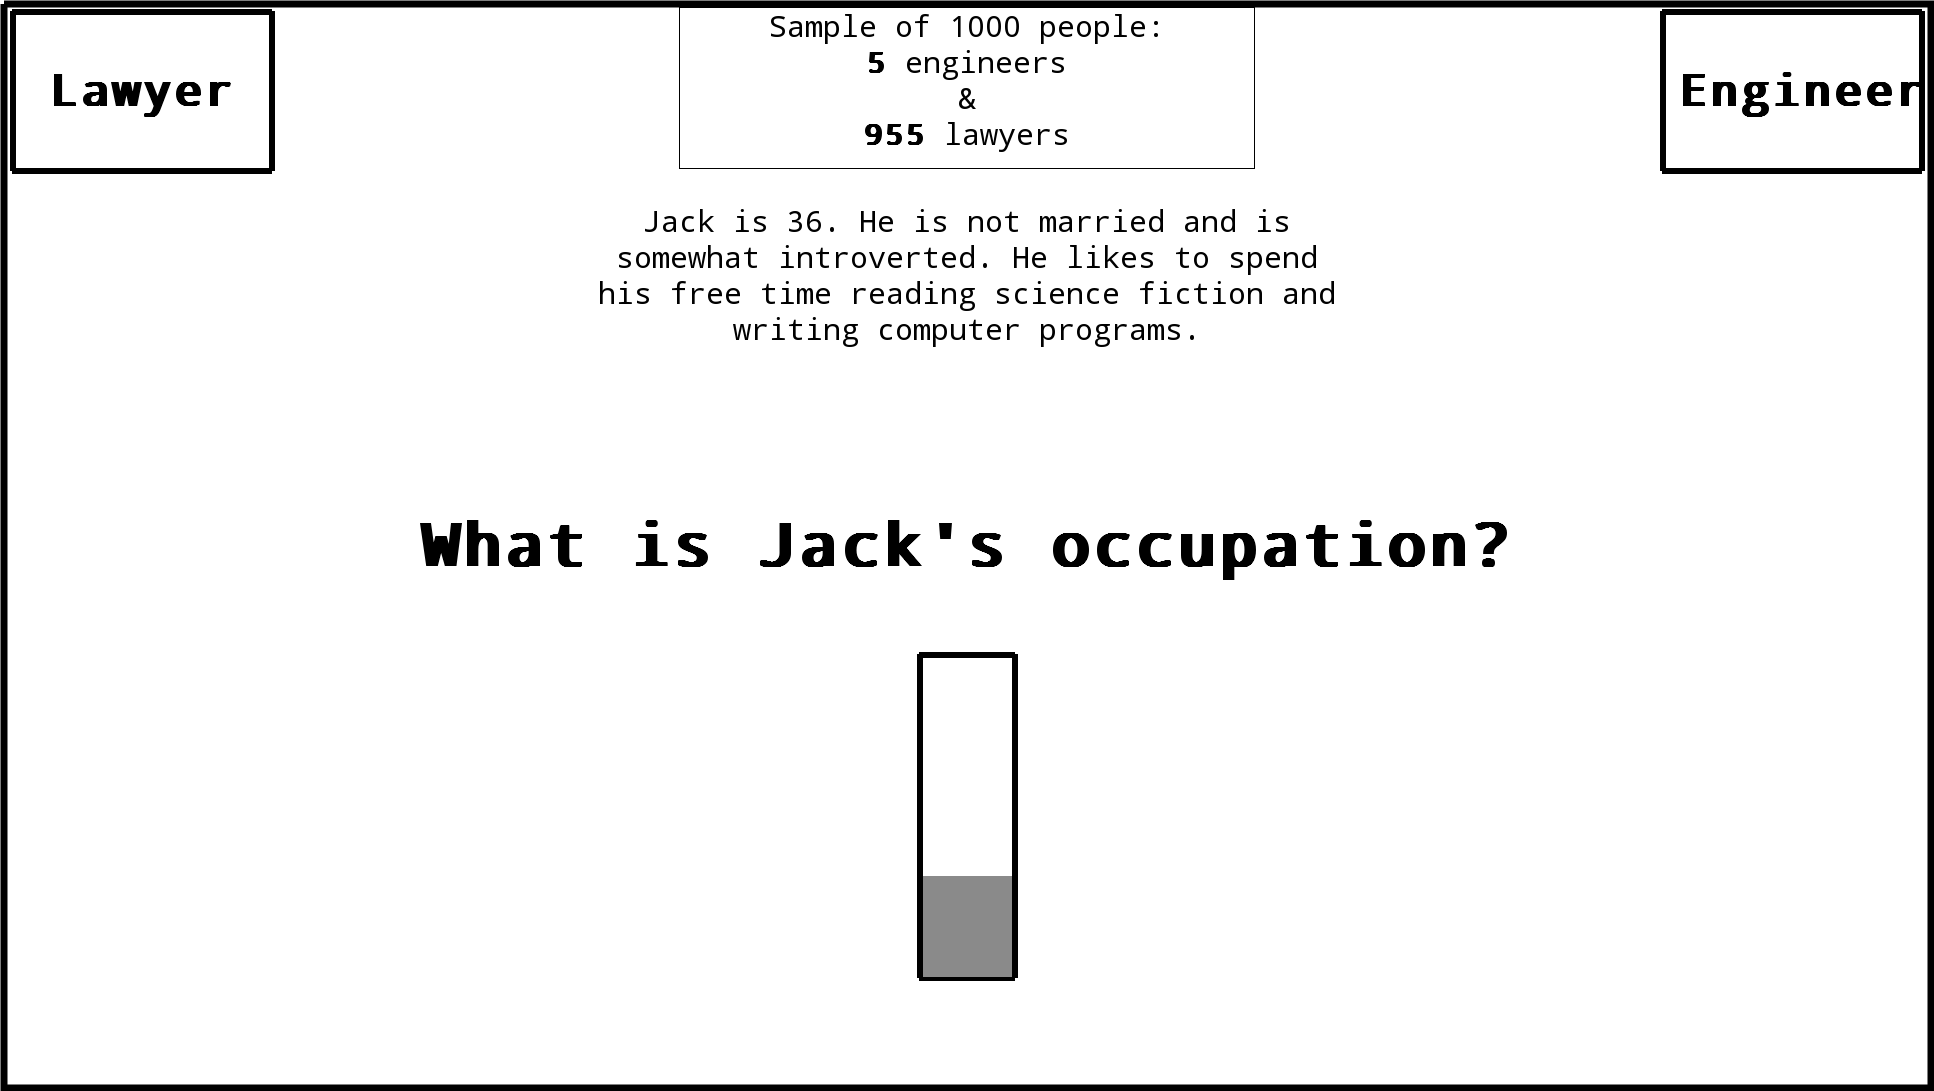
\includegraphics[width=\figurewidth]{imgs/exp5_screenshot.png}
  \caption[A screen shot from Experiment 5.]{
    \label{fig:exp5_screenshot}
    A screen shot from Experiment 5.
    The description suggests that Jack is more likely to be an engineer
    (the response option on the left),
    but the base rates suggest he is more likely to be a lawyer
    (the option on the right).
    The green timer in the centre of the screen
    is empty at the start of each trial,
    and fills up from the bottom over six seconds.
  }
\end{figure}


Following trials in which no response was given within 6 seconds (N = 2),
participants were asked to try to respond more quickly.
On trials where participants did not move the mouse cursor
from the ``NEXT'' button within 2 seconds of the onset of the probe question (N = 4),
a message reminding them that they were under time pressure
and asking them to ``try to start moving as soon as you see the target'',
was shown.

For each trial, I recorded the time taken to
finish reading the description and click on the ``NEXT'' button
(\emph{reading time}, measured from the appearance 
of the ``NEXT'' button, 5 seconds after the onset of the description itself),
the response chosen, the time from the onset of the probe text taken to respond,
and the position of the mouse cursor, sampled at 50 Hz (every 20 milliseconds).

